\documentclass[]{article}
\usepackage[T1]{fontenc}
\usepackage{lmodern}
\usepackage{amssymb,amsmath}
\usepackage{ifxetex,ifluatex}
\usepackage{fixltx2e} % provides \textsubscript
% use upquote if available, for straight quotes in verbatim environments
\IfFileExists{upquote.sty}{\usepackage{upquote}}{}
\ifnum 0\ifxetex 1\fi\ifluatex 1\fi=0 % if pdftex
  \usepackage[utf8]{inputenc}
\else % if luatex or xelatex
  \ifxetex
    \usepackage{mathspec}
    \usepackage{xltxtra,xunicode}
  \else
    \usepackage{fontspec}
  \fi
  \defaultfontfeatures{Mapping=tex-text,Scale=MatchLowercase}
  \newcommand{\euro}{€}
\fi
% use microtype if available
\IfFileExists{microtype.sty}{\usepackage{microtype}}{}
\ifxetex
  \usepackage[setpagesize=false, % page size defined by xetex
              unicode=false, % unicode breaks when used with xetex
              xetex]{hyperref}
\else
  \usepackage[unicode=true]{hyperref}
\fi
\hypersetup{breaklinks=true,
            bookmarks=true,
            pdfauthor={Angel M. Garcia},
            pdftitle={Using Subgroup Discovery algorithms in R: The SDR package},
            colorlinks=true,
            citecolor=blue,
            urlcolor=blue,
            linkcolor=magenta,
            pdfborder={0 0 0}}
\urlstyle{same}  % don't use monospace font for urls
\setlength{\parindent}{0pt}
\setlength{\parskip}{6pt plus 2pt minus 1pt}
\setlength{\emergencystretch}{3em}  % prevent overfull lines
\setcounter{secnumdepth}{0}
\usepackage{graphicx}
\usepackage[utf8]{inputenc}

\title{Using Subgroup Discovery algorithms in R: The \textbf{SDR} package}
\author{Angel M. Garcia}
\date{\texttt{r Sys.Date()}}

\begin{document}
\maketitle

\abstract{
Subgroup Discovery is a data mining task between classification and description, this task is nowadays a relevant task for researchers due to it success in many fields, especially the medical field. The SDR package provide the posibility of use some of the algorithms that exists in the specialized bibliography by means of using datasets provided in the format specified by data mining tool KEEL without dependencies to other tools/packages in the R console. Also, the package provide a graphical interface to use the algorithms easily and to do basic exploratory analysis with datasets in KEEL format.
}

\section{Introduction}\label{introduction}

Nowadays, a huge amount of information is generated everyday over the
Internet. Such information contains implicit knowledge that is very
important to many organizations because they give the possibility, for
example, of improve their products or services.\\In order to achieve
this purpose, traditional techniques of knowledge extraction like
\emph{OLAP(On-Line Analitical Processing)} are not capable to extract
knowledge as well as data mining do. Due to the success of data mining
at extracting knowledge, a lot of techniques and methods have been
designed. Such methods can be classified into two vast fields according
to their final objective:\\

\begin{itemize}

\item Predictive data mining: which objective is to find a value of a predefined variable of interest in new instances that arrive at the system.  
\item Descriptive data mining: which objective is to find relationships between instances that are at the moment in the system. 

\end{itemize}

This classification does not cover all the algorithms that exists in
data mining, and subgroup discovery is one of those fields not covered
by this classification because it has caracteristics of both fields.
Now, R has in CRAN repository a package called \emph{rsubgroup}
\cite{rsubgroup}, this package is only an interface to use the subgroup
discovery algorithms provided in VIKAMINE \cite{vikamine} data mining
tool, and has a strong dependency with this tool and use the package
\emph{rJava} \cite{rjava} that also provided an interface to use Java
files in R. So, this packages has a lot of external dependencies.

Our \textbf{SDR} package implements by now other subgroup discovery
algorithms that is not available on VIKAMINE and those algorithms are
implemented directly in R, so no dependencies with other tools/packages
are necessary to perform a subgroup discovery task and the posibilities
of growing the package by means of the adition of new algorithms is
easier for every user of R (we have a public GitHub repository where
everyone can contribute). Also our package provide a web interface
available at http://sdrinterface.shinyapps.io and locally by calling the
\texttt{SDR\_GUI()} function. Such interface could, in one hand make a
subgroup discovery task via web without having R installed in the system
or in the other hand, make an easier task by using the visual controls
of the web interface.\\Further, our package provide a function to read
KEEL \cite{keel} datasets files, a dataset format that is not supported
now in R.

\section{Subgroup Discovery}\label{subgroup-discovery}

Subgroup discovery could be defined as \cite{definicionSD}:

\begin{quote}
In subgroup discovery, we assume we are given a so-called population of
individuals (objects, customer, . . .) and a property of those
individuals we are interested in. The task of subgroup discovery is then
to discover the subgroups of the population that are statistically
``most interesting'', i.e.~are as large as possible and have the most
unusual statistical (distributional) characteristics with respect to the
property of interest.
\end{quote}

Subgroup discovery tries to find relations between different properties
of a set with respect of a target variable, but this relations must be
statistically interesting, so it is not necessary to find complete
relations but partial relations.\\The representation of thes relations
is in form of rules, one per relation. This rule can be defined as:

\begin{equation} R: Cond \rightarrow Target_{value} \end{equation}

Where $Target_{value}$ is the value for the variable of interest (target
variable) for the subgroup discovery task and $Cond$ is normally a
conjunction of attribute-value pairs which describe the characteristics
of the subgroup induced.\\Subgroup discovery is halfway between
description and classification because subgroup discovery has a target
variable but his objective is not predict but describe. Likewise the use
of a target variable is not possible in description, because description
find relations among all variables.\\A key point to understand what
subgroup discovery do is his difference with predictive data mining.
Predictive data mining tries to split the entire search space in a
normally complex way to find a value for a variable of interest in new
incoming instances while subgroup discovery tries to find interesting
relations between those instances to find what characteristics of those
instances are interesting regarding the variable of interest.\\An
example could be a group of patients and our variable of interest is if
those patients has or has not got heart disease. Predictive data mining
objective is to predict if new patients will have a heart disease by
their characteristcs while subgroup discovery tries to find what
subgroup of patients are more likely to have a heart disease and with
those characteristics, make a treatment against those characteristics.

\subsection{Main elements of subgroup discovery
algorithms}\label{main-elements-of-subgroup-discovery-algorithms}

All the algorithms that are included into this data mining task must
have the next characteristics:

\begin{itemize}
  
  \item Type of target variable: The target variable could be binary (two posible values), categorical ( $n$ posible values) or numerical (a real value within a range).
  \item Description language: Rules must be as simple as possible. Due to this, rules are composed normally by conjunctions of attribute-value pairs or in disyuntive normal form. Also, to improve the interpretability of the results, fuzzy logic could be used.
  \item Quality measures: Are very important because they define when a subgroup is "interesting". They will be briefly described below.
  \item Search strategy: The search space grows exponentially by the number of variables. Using a search strategy that could find a good solution or the optimal one without searching into the whole search space is important.
  
\end{itemize}

\subsection{Quality measures for subgroup discovery
\label{medidas}}\label{quality-measures-for-subgroup-discovery}

A lot of quality measures have been defined for this task and there is
no consensus for what quality measure it is the best for the task. The
most important quality measures for subgroup discovery are described
below\cite{kais}:

\begin{itemize}
  
  \item $N_r$: The number of rules generated.
  \item $N_v$: The average number of variables that the rules generated have.
  \item \textbf{Support:} It measures the frequency of correctly classified examples covered by the rule: \begin{equation} Sup(x)= \frac{n(Cond \wedge  T_v)}{n_s} \label{support} \end{equation} Where $n(Cond \wedge  T_v)$ means the number of correctly covered examples  and $n_s$ is the number of examples in the dataset.  
  \item \textbf{Coverage:} It measures the percentage of examples covered by the rule related to the total number of examples: \begin{equation} Cov(x)= \frac{n(Cond)}{n_s} \label{coverage} \end{equation} where $n(Cond)$ means the number of covered examples by the rule.
  \item \textbf{Confidence:} It measure the percentage of examples correctly covered of the total of covered examples: \begin{equation} Conf(x) = \frac{n(Cond  \wedge Target_{value})}{n(Cond)} \label{confidence} \end{equation}
  \item \textbf{Interest:} It measures the interest of the rule determined by the antecedent and consequent: \begin{equation} Int(x) = \frac{\sum_{i = 1}^{n_v}Gain(A_i)}{n_v \cdot log_2(|dom(G_k)|)} \label{Interest} \end{equation} where $Gain$ is the information gain, $A_i$ is the number of values of the variable and $|dom(G_k)|$ is the cardinality of the target variable.
  \item \textbf{Significance:} It reflects the novelty in the distribution of the examples covered by the rule regarding the whole dataset: \begin{equation} Sign(x) = 2 \cdot \sum_{k=1}^{n_c}n(Cond \wedge T_{vk}) \cdot log(\frac{n(Cond \wedge T_{vk})}{n(Cond \wedge T_v) \cdot p(Cond)}) \label{Significance} \end{equation} where $p(Cond) = \frac{n(Cond)}{n_s}$
  \item \textbf{Unusualness:} It is defined as the weigthed relative accuracy of a rule \begin{equation} WRAcc(x) = \frac{n(Cond)}{n_s}(\frac{n(Cond \wedge T_v)}{n(Cond)} - \frac{n(T_v)}{n_s})\label{Unusualness} \end{equation} where $n(T_v)$ is the number of examples that belong to the target variable.
  
\end{itemize}

\section{Algorithms of the package}\label{algorithms-of-the-package}

Now, we describe the algorithms that are available in our package. This
contains three algorithms: SDIGA \cite{sdiga}, MESDIF \cite{mesdif} and
NMEEF-SD \cite{nmeef}. In chapter \ref{uso} we describe how to use the
algorithms.

\subsection{SDIGA (Subgroup Discovery Iterative Genetic
Algorithm)}\label{sdiga-subgroup-discovery-iterative-genetic-algorithm}

The algorithm SDIGA is a subgroup discovery algorithm that extract rules
with two possible representations: one with conjunctions of
attribute-value pairs (called canonical representation) or one with a
disyuntive normal form (DNF) in the antecedent. It follows an iterative
schema with a genetic algorithm in his core to extract those rules, this
genetic algorithm only extract one rule, the best of the population, and
after the extraction a local optimization could be performed in order to
improve the generality of the rule. As the algorithm follows an
iterative schema, the genetic algorithm is executed one time after
another until a stopping criteria is reached: the rule obteined by the
genetic algorithm and after the local improvement phase must cover at
least one example not covered by precedent rules and this rule must have
a minimum confidence (see Equation \ref{confidence}).\\SDIGA can work
with lost data (represented by the maximum value of the variable + 1),
categorical variables and numerical ones using fuzzy logic with the
latter to improve the interpretability of the results.

\subsubsection{Components of genetic algorithm of
SDIGA}\label{components-of-genetic-algorithm-of-sdiga}

As we mentioned above, a genetic algorithm is the core of SDIGA. Such
genetic algorithm is the responsible of extract one rule per execution
and this rule it is the best of the population at the final of the
evolutive process.

\paragraph{Representation schema
\label{esquemas}}\label{representation-schema}

Each chromosome in the population represents a possible rule but it only
represents the antecedent part of the rule because the consecuent is
prefixed. SDIGA can handle two types of representation as we mentioned
above, canonical and DNF.\\Canonical representation is formed by a
numerical vector of a fixed length equal to the number of variables with
possibles values in a range in $[0, max]$ where $max$ is the number of
possible values for categorical variables or the number of fuzzy sets
defined for numerical variables. This $max$ value represents the no
participation of that variable in the rule.\\DNF representation is
formed by a binary vector, also with fixed length equal to the sum of
all number of values/fuzzy sets of the variables. Here, a variable does
not participate in a rule when all of his values are equal to zero or
one.

\paragraph{Crossover operator \label{cruce}}\label{crossover-operator}

SDIGA follows a pure stationary schema which only crosses the two best
chromosomes in an iteration of the evolutionary process. This crossover
is performed by a two-point cross operator.

\paragraph{Mutation operator \label{mutacion}}\label{mutation-operator}

Mutation operator is applied over all the population of parents and
chromosomes generated by crossover. The mutation probability is applied
at every gene. This operator can be applied in two ways (both with the
same probability):

\begin{itemize}
\item Eliminate the variable: it puts the no participation value in that variable.
\item Put a random value: it puts a random value in that variable. The no participation value is also included.
\end{itemize}

\paragraph{Fitness function}\label{fitness-function}

The function to define the quality of a chromose in SDIGA is a weighted
average of three of the quality measures described in section
\ref{medidas}. So the functions to maximize is:

\begin{equation} f(x) = \frac{Sop(x) \cdot  w_1 + Conf(x) \cdot w_2 + Obj3(x) \cdot  w_3}{\sum_{i=1}^{3} w_i} \label{fitnessSDIGA} \end{equation}

where:

\begin{itemize}
 \item $Sop(x)$ is the local support. This support is a modification of support (see Equation \ref{support}) and can be crisp or fuzzy: 
    \begin{itemize}
      \item Crisp Support: \begin{equation} Sop_n(x) = \frac{Ne^+(R_i)}{Ne_{NC}} \end{equation}
      \item Fuzzy Support: \begin{equation} Sop_d(x) = \frac{\sum_{k} APC(E^k, R_i)}{Ne_{NC}} \end{equation}
      where $Ne^+(R_i)$ is the number of examples covered by the rule and it is not covered by previous rules. $Ne_{NC}$ is the number of examples of the target variable that it is not covered by any rule yet and $APC$ is the \textit{Antecedent Part Compatibility} equation calculted only with new covered examples (see Equation \ref{APC}).
    \end{itemize}
    
    \item $Conf(x)$ is the confidence defined as in Equation \ref{confidence} for the crisp case, but for fuzzy case is defined as the ratio of the sum of $APC$ expresion of the correctly covered examples and the sum of $APC$ all examples covered by the rule: \begin{equation} Conf_d(x) = \frac{\sum_{E^{CC}} APC(E^k, R_i)}{\sum_{E^{C}} APC(E^k, R_i)} \end{equation} where $E^{CC}$ are the correctly covered examples and $E^C$ are the covered examples.
    
    \item $Obj3(x)$ is other quality measure of section \ref{medidas}
    \item $w_i$ is the weight of objective \textit{i}
\end{itemize}

As this rules uses fuzzy logic, we need an expresion to determine when
an example is covered or not by a rule and also determine the belonging
degree of that example to the rule. This function is determined by the
expression $APC$ (\emph{Antecedent Part Compatibility}) and it is
calculate by the expresssion:

\begin{equation} APC(e, R_i) = T(TC(\mu _{1}^{1}(e_1), ... , \mu _{n}^{1}(e_i)), ... , TC(\mu _{1}^{i}(e_1), ... , \mu _{n}^{i}(e_i))) \label{APC} \end{equation}

where:

\begin{itemize}
  \item $e_i$ is the value of the example for the variable \textit{i}
  \item $\mu_{n}^{i}$ is the belonging degree to the set \textit{n} of the variable \textit{i}
  \item $TC$ is the fuzzy t-conorm. In this case is the maximum t-conorm.
  \item $T$ is the fuzzy t-norm. In this case is the minimum t-norm.
\end{itemize}

$\mu_{n}^{i}$ will be one or zero if the variable is categorical and its
value is the same of the rule or not. In case of numerical variable,
$\mu_{n}^{i}$ will be calculated following the triangular belonging
degree function.

\begin{equation} 
\mu_{a,b,c} = \left\{\begin{matrix}
0 & x \leq a\\ 
\frac{x-a}{b-a} &  a \leq x \leq b\\ 
 \frac{c-x}{c-b}&  b \leq  x \leq  c\\ 
 0 &   c \leq  x
\end{matrix}\right.
\end{equation}

\paragraph{Replace operator}\label{replace-operator}

To get next population for the next iteration a replace operator must be
performed. This operator sort the population by fitness value and keep
only the \emph{n} best chromosomes, being \emph{n} the size of the
population.

\subsubsection{Local optimization}\label{local-optimization}

After the genetic algorithm returns a rule, this rule could be improved
by means of a local optimization based on a \emph{hill climbing first
best} local search. The algorithm eliminate one by one a variable and if
the rule has a support and confidence greater than or equal the actual,
the process starts again with that variable eliminated.

\subsection{MESDIF (Multiobjetive Evolutionary Subgroup DIscovery Fuzzy
rules)}\label{mesdif-multiobjetive-evolutionary-subgroup-discovery-fuzzy-rules}

MESDIF is a multi-objective genetic algorithm that extract fuzzy rules.
The representation used could be canonical or DNF (see Section
\ref{esquemas}). This algorithm follows the SPEA2 \cite{spea} approach
where an elite population is used along the whole evolutive process. At
the end of the process, the rules stored in the elite population where
returned as result.\\The multi-objective approach is based on a niches
schema based on the dominance in the Pareto front. This schema allows to
find non-dominated individuals to fill the elite population, that has a
fixed size. In Figure \ref{MESDIFEsquema} we see a basic schema of the
algorithm.

\begin{figure}[htbp]
  \centering 
  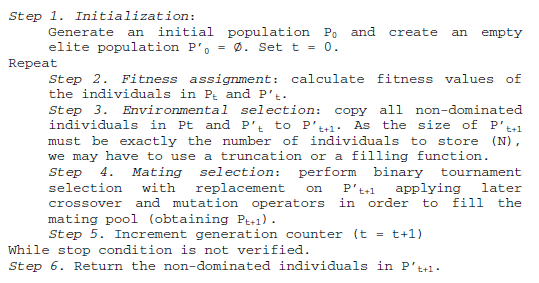
\includegraphics{MESDIFSchema.png}
  \caption{MESDIF operations schema}
  \label{MESDIFEsquema}
\end{figure}

\subsubsection{Components of the genetic
algorithm.}\label{components-of-the-genetic-algorithm.}

Now we describe briefly the components of the genetic algorithm to show
how it works.\pagebreak

\paragraph{Initial Population generation
\label{biasedInit}}\label{initial-population-generation}

The initial population operator performed by MESDIF produce random
chromosomes in two ways: one percentage of chromosomes are produced
ramdomly and the rest are produced also randomly, but with the
difference that only a maximum number of variables could participate in
the rule. This produce more generality in the generated rules.

\paragraph{Fitness function}\label{fitness-function-1}

To obtain the fitness value of each chromosome, MESDIF follows this
steps:

\begin{itemize}

\item First, we look for dominated and non-dominated individuals in both populations. We call \textit{strength of an individual} the number of individuals that this domain.
\item An initial fitness value $A_i$ is calculated for each individual, such value is the sum of the strength of all dominators of individual \textit{i}. So, we have to minimize this value and for non-dominated individuals is zero.
\item Due to this system could fail if there are a lot of non-dominated individuals, additional information about density is included. This density is computed by the nearest neighbour approach and it is calculate by \begin{equation} D(i) = \frac{1}{\sigma^k + 2} \end{equation} where $\sigma^k$ is the k-th nearest neighbour.
\item The final adaptation value is the sum of initial fitness and density information \begin{equation} Fitness(i) = D(i) + A(i) \label{fitnessMESDIF} \end{equation}

\end{itemize}

\paragraph{Truncation operator}\label{truncation-operator}

As the elite population has a fixed size, we need a truncation operator
to truncate the elite population if all non-dominated individuals can
not fit in elite population. To make this truncation, the operator take
all non-dominated individuals and calculate the distance among every
one. Then, the two closest individuals are taken and eliminate the
individual with his k-th nearest neighbour with a minor distance. This
process is repeated until non-dominated indivuals fit in elite
population.

\paragraph{Fill operator}\label{fill-operator}

If the number of non-dominated individuals are less than the size of the
elite population, we need to fill elite population with dominated
individuals. The operator sort the individuals by its fitness value and
copy the \emph{n} first individuals to elite population, where \emph{n}
is the size of the elite population.

\paragraph{Genetic operators}\label{genetic-operators}

The genetic operators of MESDIF are:

\begin{itemize}
  \item A two-point crossover operator (see Section \ref{cruce})
  \item A biased mutation operator, the functionality is the same operator of SDIGA (see Section \ref{mutacion}) but it is applied over a population of selected individuals.
  \item A selection operator based in a binary tournament selection. This selection is only applied over the individuals of elite population.
  \item A replacement of the selected population based on the direct replace of the \textit{k} worse individuals of the population. \textit{k} is the number of individuals returned after crosses and mutations.
\end{itemize}

\subsection{NMEEF-SD (Non-dominated Multi-objective Evolutionary
algorithm for Extracting Fuzzy rules in Subgroup
Discovery)}\label{nmeef-sd-non-dominated-multi-objective-evolutionary-algorithm-for-extracting-fuzzy-rules-in-subgroup-discovery}

NMEEF-SD is another multi-objectve genetic algorithm based in the
NSGA-II \cite{nsga} approach. This algorithm has a fast sorting
algorithm and a reinitialisation based on coverage if the population
does not evolve for a period.\\This algorithm only works with a
canonical representation (see Section \ref{esquemas}). In
\cite{estudioNMEEF} a study is presented where it reflects the low
quality of rules obtained with a DNF representation.

\subsubsection{Evolutionary process}\label{evolutionary-process}

The evolutionary process follows this steps

\begin{itemize}
  \item An initial biased population $P_t$ is generated (see Section \ref{biasedInit}).
  \item The genetic operators are applied over $P_t$ obtaining $Q_t$ with the same size as $P_t$.
  \item $P_t$ and $Q_t$ are joined obtaining $R_t$ and the fast sorting algorithm is applied over $R_t$. The individuals are sorted forming different fronts in the following way: "The first front ($F_1$) is composed of non-dominated individuals, the second front ($F_2$) is composed by individuales dominated by one individual; the third front ($F_3$) is composed by individuals dominated by two, and so on."
  \item After that, the algorithm generates the population of the next generation ($P_{t+1}$). First, the algorithm checks if the Pareto front covers new examples as it can be show in Figure \ref{procesoNMEEF}. If this condition is not satisfied during a period of the evolutionary process, a reinitialisation based on coverage is performed. Otherwise, the algorithm gets the next population ($P_{t+1}$) introducing, in order, the first complete fronts of $R_t$. If the last front does not fit completely in $P_{t+1}$ then, the front is sorted by the \textit{crowding distance} and first individuals are copied until $P_{t+1}$ is filled.
  \item At the final of the evolutionary process the individuals in the Pareto front are returned.
\end{itemize}

\begin{figure}[hbtp]
  \centering
  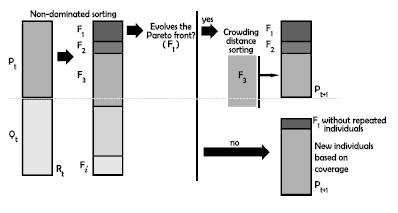
\includegraphics{NMEEFSchema.png}
  \caption{Operation schema of NMEEF-SD}
  \label{procesoNMEEF}
\end{figure}

\subsubsection{Genetic operators}\label{genetic-operators-1}

The genetic operators of NMEEF-SD are a two-point crossover operator
(see Section \ref{cruce}) and a biased mutation operator (see Section
\ref{mutacion}).

\subsubsection{Reinitialisation
operator}\label{reinitialisation-operator}

This operator is applied if the Pareto front does not cover any new
example during a 5\% of the total number of evaluations. Then, the
algorithm copy the non duplicated individuals in the Pareto front to
$P_{t+1}$ and the rest of individuals are generated by means of trying
to cover one example of the target class with a maximum number of
variables.

\section{Use of SDR package} \label{uso}

In this section we are going to explain how to use this package. This
package tries to use in a really simple way subgroup discovery
algorithms and also without any dependencies.

\subsection{Installing and load the
package.}\label{installing-and-load-the-package.}

The package SDR is now available at CRAN servers, so it can be installed
as any other package by simply typing:
\texttt{\{r,eval=FALSE\} install.packages("SDR")} Also, the develop
version is available into GitHub at http://github.com/aklxao2/SDR, feel
free to clone and contribute if you wish. If you wish to use the
development version you need to install the package \texttt{devtools}
using the commando \texttt{install\_github}:
\texttt{\{r,eval=FALSE\} devtools::install\_github('aklxao2/SDR')}
\textbf{SDR} depends only on the package \textbf{shiny} \cite{shiny}.
This package is neccesary to use the user interface in a local
way.\\Once installed the package has to be loaded before use it. The
package can be loaded through \texttt{library()} or \texttt{require()}.
After loading the package there are six datasets available:
\texttt{carTra}, \texttt{carTst}, \texttt{germanTra},
\texttt{germanTst}, \texttt{habermanTra} and \texttt{habermanTst} that
corresponds to \texttt{car}, \texttt{german} and \texttt{haberman}
training and test datasets.\\This package use an internal representation
assigned to the \texttt{"keel"} class . All the information about the
datasets are available in this class.

\subsection{Load a KEEL dataset}\label{load-a-keel-dataset}

To use the algorithms available in this package, we could load a dataset
if it is different of the three examples availables. Assuming the files
\texttt{'irisTra.dat'} and \texttt{'irisTst.dat'}, corresponding to the
classical iris dataset, the load of this files will be as follows:
\texttt{\{r,eval=FALSE\} irisTraining \textless{}- read.keel("irisTra.dat") irisTest \textless{}- read.keel("irisTst.dat")}
As we mentioned above, the algorithms in the package uses fuzzy logic,
and the definitions of the fuzzy sets are implicit to every dataset.
This fuzzy sets definitions are defined with the same length and the
same type (all are triangular fuzzy sets). By default, the function
\texttt{read.keel()} creates three fuzzy sets for every variable. To
change the number of sets per variable, you can use the argument
\texttt{'nLabels'}:
\texttt{\{r,eval=FALSE\} irisTraining \textless{}- read.keel("irisTra.dat", nLabels = 5) irisTest \textless{}- read.keel("irisTst.dat", nLabels = 5)}

If you want to get more KEEL datasets format, please visit:
http://sci2s.ugr.es/keel/datasets.php

\subsection{Modify properties of a loaded KEEL
dataset}\label{modify-properties-of-a-loaded-keel-dataset}

Once we loaded a dataset, we can modify some characteristics of its
properties using this functions of the package.

\begin{itemize}
  \item \textbf{changeTargetVariable:} The subgroup discovery algorithms take as target variable the last variable defined in the dataset. If this is not our target variable we need to change it by means of this function that needs a dataset to change and the position of the target variable. This target variable must be categorical. So, if the variable is numeric, this functions throws an error.

  \item \textbf{modifyFuzzyCrispIntervals:} This functions allows to modify the number of fuzzy sets that there are in a dataset. This is useful when we are looking for the best number of fuzzy sets in our experimentations. We only need to specify the dataset we want to modify and the new number of fuzzy sets.
  \end{itemize}

\texttt{\{r,eval=FALSE\} irisTraining \textless{}- changeTargetVariable(dataset = irisTraining, posVariable = 2) carTra \textless{}- changeTargetVariable(dataset = carTra, posVariable = 2)}

\texttt{\{r,eval=FALSE\} irisTraining \textless{}- modifyFuzzyCrispIntervals(dataset = irisTraining, nLabels = 7)}

\subsection{Executing Subgroup Discovery
algorithms}\label{executing-subgroup-discovery-algorithms}

Once our datasets are ready to be used, it is time to execute one
subgroup discovery algorithm. For example we want to execute the
algorithm MESDIF. For the rest of the algorithm this steps are equal and
only a few parameters are diferent, if you need help with the
parameters, refer to the help of the function using
\texttt{help(function)} or \texttt{?function}.\\The subgroup discovery
algorithms have two ways of execution: one of them is by indicating the
path of a parameters file, with all the neccesary parameters. The other
is by putting in the function all parameters one by one. The first mode
of use is indicated when we have a dataset prepared for executing
directly because this way does not allow us to modify the properties of
the dataset, so the second way is indicated when we load and/or modify a
dataset before execute the algorithm.\\When we execute the algorithm,
the results are shown in the console. This results are divided in three
fields:

\begin{itemize}
\item First, an echo of the parameters used in the execution are shown.
\item Second, the subgroups or rules genereted by the algorithm.
\item Finally, some quality measures about the rules generated applied to test data are shown. The final value are a summary of this quality measures for all rules
\end{itemize}

As the results line could be extremly large, the algorithms also save
this results into three files, divided in the same categories described
above.
\texttt{\{r,eval=FALSE\} MESDIF(paramFile = "MESDIFparameters.txt")}
\texttt{\{r,highlight=TRUE\} library("SDR") MESDIF( paramFile = NULL,         training = habermanTra,         test = habermanTst,         output = c("optionsFile.txt", "rulesFile.txt", "testQM.txt"),         seed = 0,         nLabels = 3,         nEval = 300,         popLength = 100,         eliteLength = 3,         crossProb = 0.6,         mutProb = 0.01,         RulesRep = "can",         Obj1 = "CSUP",         Obj2 = "CCNF",         Obj3 = "null",         Obj4 = "null",         targetClass = "positive"         )}

\section{The user interface}\label{the-user-interface}

As we mentioned at the begin of this paper, the \textbf{SDR} package
provide to the user an interface to use the subgroup discovery task in a
more easy way and also do some basic exploratory analysis tasks.\\We can
use the user interface by two ways: one of them is using the interface
via web at: http://sdrinterface.shinyapps.io/shiny . This has the
advantage of use the algorithm without having R installed in our system
and also avoid expending process time in our machine. The other way is
to use the interface is in a local way, having our local server. This
could be possible simply using: \texttt{\{r,eval=FALSE\} SDR\_GUI()}
This function launch the user interface in our predetermined web
browser. As we can see in Figure \ref{pantallaInicial}. The page are
organized into an options panel at the left and a tabbed panel at the
right. Here is where our results are shown when we execute the
algorithms.\\The first we have to do is to load a KEEL dataset. If we
want to execute a subgroup discovery algorithm we must load a training
and a test file \textbf{having the same} \texttt{'@relation'}
\textbf{field in the KEEL dataset file.}\\Once we select the dataset,
automatically it shows a graph with information about the last variable
defined in the dataset. The graph shows the distribution of examples
having some values of the variable. At the rigth of this graphic we can
see a table with some basic information, more extended if this variable
is numerical.

\begin{figure}[hbtp]
  \centering
  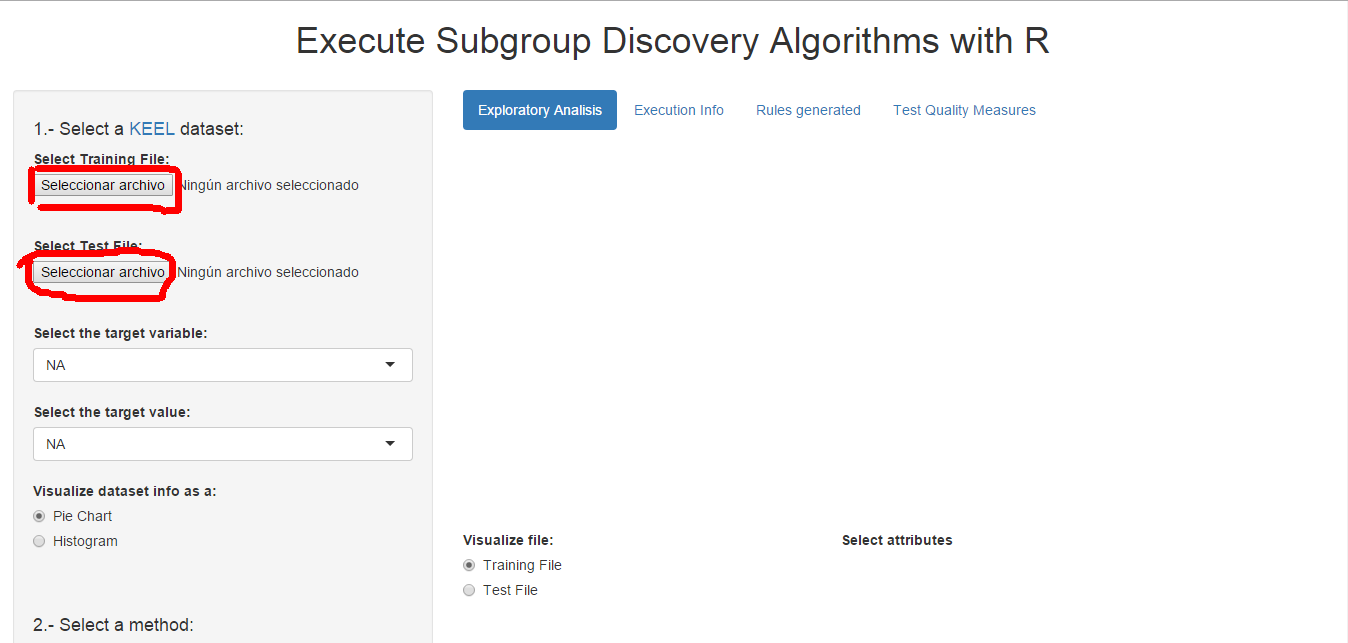
\includegraphics[width=0.8\linewidth]{Interfaz1.png}
  \caption{Initial screen of the SDR user interface.}
  \label{pantallaInicial}
\end{figure}

\pagebreak
When loaded a dataset we can do a lot of things, in Figure
\ref{pantalla2} we can see all the possibilities we can do:

\begin{enumerate}
\item As we mentioned above, we can load a second dataset as a test (or training) file.
\item This lists have a double function. In one hand we could select the variable to visualize in the graph and in the other hand is to select the target variable for executing a subgroup discovery algorithm. Below the variable selection we can choose a target value of the variable to find subgroups about this value or search for all posible values of the target variable.
\item Here we can choose how the information will be visualized, for categorical variables we can choose show the information as a pie chart or as a historgram, for numerical variables only histogram is available.
\item Here we can choose the subgroup discovery algorithm  and his parameters, that it is shown below. Below the parameters, we have the button to execute the subgroup discovery algorithm.
\item This section allows the selection, for categorical variables, the values of that variable has that we can see in the graph. It is important to remark that it only "hide" the values in the graph, so it does not eliminate any example of the dataset.
\item It allows to visualize information about the training or test file.
\end{enumerate}

\begin{figure}[hbtp]
  \centering
  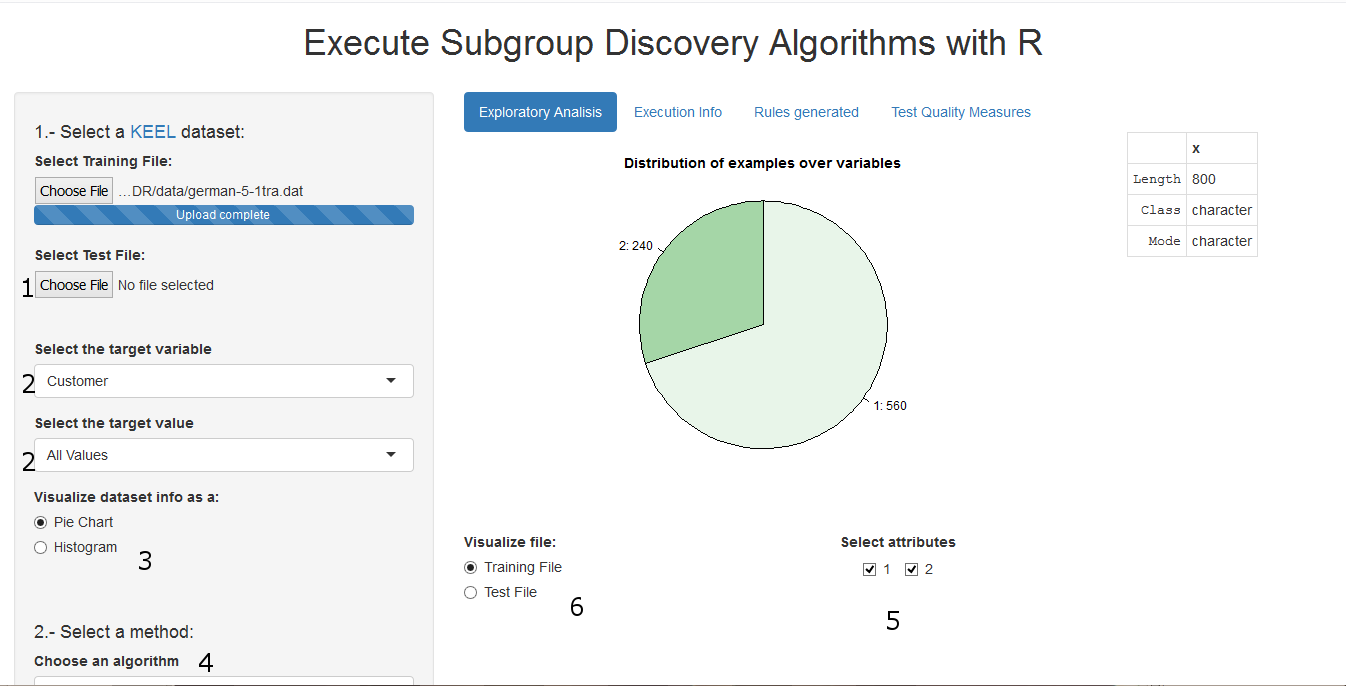
\includegraphics[width=0.8\linewidth]{Interfaz2.png}
  \caption{Screen of the user interface once loaded a dataset.}
  \label{pantalla2}
\end{figure}

After the execution of a subgroup discovery algorithm, we go
automatically to the tab \texttt{'Rules generated'}, this tab contains a
table with all subgroups generated. If we want we could filter rules by
variable, for example, typing into the \texttt{'Search'} field.\\The tab
\texttt{'Execution Info'} shows an echo of the parameters used for
launch the algorithm. This echo is equal than the one we can see in R
console.\\The tab \texttt{'Test Quality Measures'} shows a table with
quality measures of every rule applied to test dataset. The last row its
a summary of results and shows the number of rules we have and the
average results of every quality measure.

\section{Summary}\label{summary}

In this paper the \textbf{SDR} package has been introduced. This package
can use three subgroup discovery algorithms without any other
dependencies to others tools/packages. Also, the posibility of read and
load datasets in the KEEL dataset format is provided. The package also
implements a few tools to prepare the dataset to be used by a subgroup
discovery algorithm. Finally, a web-based interface is developed for
make the work easier, even if we do not have R installed in our
system.\\The devolpment of the package will continue in the future,
including more functionality to work with KEEL datasets, adding new
subgroup discovery algorithms and also improve the web interface. As we
can see we have a great job ahead, so we encourage other developers to
participe adding tools or algorithms into the package, as we will do in
futures releases.

\begin{thebibliography}{20}


\bibitem[Wrobel S. (2001)]{definicionSD}
\newblock \emph{Inductive logic programming for knowledge discovery in databases. }
\newblock Springer, chap Relational Data Mining, pp 74-101.

\bibitem[Martin Atzmueller, (2014)]{rsubgroup}
\newblock \emph{rsubgroup: Subgroup Discovery and Analytics.}
\newblock URL \url{http://CRAN.R-project.org/package=rsubgroup}

\bibitem[Simon Urbanek (2013)]{rjava}
\newblock \emph{rJava: Low-level R to Java interface.}
\newblock URL \url{http://CRAN.R-project.org/package=rJava}

\bibitem[Chang(2015)]{shiny}
W.~Chang.
\newblock \emph{shiny: Web Application Framework for R}, 2015.
\newblock URL \url{http://CRAN.R-project.org/package=shiny}.
\newblock R package version 0.11.

\bibitem[M. Atzmueller, F. Lemmerich (2012)]{vikamine}
\newblock \emph{VIKAMINE - Open-Source Subgroup Discovery, Pattern Mining and Analytics}
\newblock in \emph{Machine Learning and Knowledge Discover in Databases}
\newblock pp. 842-845

\bibitem[J. Alcala-Fdez et~al.(2011)] {keel} 
\newblock J. Alcala-Fdez, A. Fernandez, J. Luengo, J. Derrac, S. Garcia, L. Sanchez, F. Herrera.
\newblock \emph{KEEL Data-Mining Software Tool: Data Set Repository, Integration of Algorithms and Experimental Analysis Framework.}
\newblock In \emph{ Journal of Multiple-Valued Logic and Soft Computing 17:2-3 (2011) 255-287}.

\bibitem[F. Herrera et~al. (2010)]{kais}
\newblock F. Herrera, M. J. del Jesus, P. Gonzalez, C. J. Carmona.
\newblock \emph{An overview on subgroup discovery: foundations and applications.}
\newblock In \emph{Knowledge and Information Systems.}
\newblock December 2011, Volume 29, Issue 3, pp 495-525.

\bibitem[M. del Jesus et~al. (2007)]{sdiga}
\newblock M. del Jesus, P. Gonzalez, F. Herrera, M. Mesonero.
\newblock \emph{Evolutionary fuzzy rule induction process for subgroup discovery: a case study in marketing.}
\newblock In \emph{IEEE Trans Fuzzy Syst.} pp. 15(4):578-592, 2007.

\bibitem[C.J. Carmona et~al. (2010)]{nmeef}
\newblock C. J. Carmona, P. Gonzalez, M. J. del Jesus, F. Herrera.
\newblock \emph{NMEEF-SD: Non-dominated Multi-objective Evolutionary algorithm for Extracting Fuzzy rules in Subgroup Discovery.}
\newblock In \emph{Fuzzy Systems, IEEE Transactions.}
\newblock Volume:18, Issue:5, pp.958-970, 2010

\bibitem[M. del Jesus et~al. (2007)]{mesdif}
\newblock M. del Jesus, P. Gonzalez, F. Herrera.
\newblock \emph{Multiobjective genetic algorithm for extracting subgroup discovery fuzzy rules.}
\newblock In \emph{Proceedings of the IEEE symposium on computational intelligence in multi-criteria decision making.} pp. 50-57, 2007

\bibitem[E. Zitzler et~al. (2001)]{spea}
\newblock E. Zitzler, M. Laumanns, L. Thiele.
\newblock \emph{SPEA2: Improving the Strength Pareto Evolutionary Algorithm.}
\newblock 2001

\bibitem[K. Deb et~al. (2000)]{nsga}
\newblock K. Deb, S. Agrawal, A. Pratap, T. Mayerivan.
\newblock \emph{A Fast Elitist Non-Dominated Sorting Genetic Algorithm for Multi-Objective Optimization: NSGA-II}
\newblock 2000

\bibitem[C. Carmona et~al. (2009)]{estudioNMEEF}
\newblock C. Carmona, P. Gonzalez , M. del Jesus, F. Herrera.
\newblock \emph{An analysis of evolutionary algorithms with different types of fuzzy rules in subgroup discovery.} 
\newblock In \emph{IEEE International Conference on Fuzzy Systems (FUZZ-IEEE).}
\newblock ICC Jeju, Jeju Island, Korea, 2009

\end{thebibliography}

\end{document}
